%%%%%%%%%%%%%%%%%%%%%%%%%%%%%%%%%%%%%%%%%%%%%%%%%%%
%% LaTeX book template                           %%
%% Author:  Amber Jain (http://amberj.devio.us/) %%
%% License: ISC license                          %%
%%%%%%%%%%%%%%%%%%%%%%%%%%%%%%%%%%%%%%%%%%%%%%%%%%%

\documentclass[a4paper,11pt]{book}
\usepackage[margin=1.5in]{geometry}
\usepackage[T1]{fontenc}
\usepackage[utf8]{inputenc}
\usepackage{lmodern}
%%%%%%%%%%%%%%%%%%%%%%%%%%%%%%%%%%%%%%%%%%%%%%%%%%%%%%%%%
% Source: http://en.wikibooks.org/wiki/LaTeX/Hyperlinks %
%%%%%%%%%%%%%%%%%%%%%%%%%%%%%%%%%%%%%%%%%%%%%%%%%%%%%%%%%
\usepackage{hyperref}
\usepackage{graphicx}
\usepackage[english]{babel}
\usepackage{amsthm}
\usepackage{mathtools}
\DeclarePairedDelimiter\ceil{\lceil}{\rceil}
\DeclarePairedDelimiter\floor{\lfloor}{\rfloor}


\newcommand{\code}{\lstinputlisting}
\newtheorem{prob}{Problem}
\let\oldprob\prob
\renewcommand{\prob}{\oldprob\indent\\}
\newtheorem*{sol}{Solution}
\let\oldsol\sol
\renewcommand{\sol}{\oldsol\normalfont}
\usepackage{listings}
\usepackage{courier}
\lstset{
	basicstyle=\footnotesize\ttfamily, % Standardschrift
	%numbers=left,               % Ort der Zeilennummern
	numberstyle=\tiny,          % Stil der Zeilennummern
	%stepnumber=2,               % Abstand zwischen den Zeilennummern
	numbersep=5pt,              % Abstand der Nummern zum Text
	tabsize=4,                  % Groesse von Tabs
	extendedchars=true,         %
	breaklines=true,            % Zeilen werden Umgebrochen
	keywordstyle=\color{red},
	frame=bt,         
	%        keywordstyle=[1]\textbf,    % Stil der Keywords
	%        keywordstyle=[2]\textbf,    %
	%        keywordstyle=[3]\textbf,    %
	%        keywordstyle=[4]\textbf,   \sqrt{\sqrt{}} %
	stringstyle=\color{white}\ttfamily, % Farbe der String
	showspaces=false,           % Leerzeichen anzeigen ?
	showtabs=false,             % Tabs anzeigen ?
	xleftmargin=17pt,
	framexleftmargin=17pt,
	framexrightmargin=5pt,
	framexbottommargin=4pt,
	%backgroundcolor=\color{lightgray},
	showstringspaces=false      % Leerzeichen in Strings anzeigen ?        
}
\lstloadlanguages{% Check Dokumentation for further languages ...
	%[Visual]Basic
	%Pascal
	C
	%C++
	%XML
	%HTML
	%Java
}
%\DeclareCaptionFont{blue}{\color{blue}} 

%\captionsetup[lstlisting]{singlelinecheck=false, labelfont={blue}, textfont={blue}}
\usepackage{caption}
\DeclareCaptionFont{white}{\color{white}}
\DeclareCaptionFormat{listing}{\colorbox[cmyk]{0.43, 0.35, 0.35,0.01}{\parbox{\textwidth}{\hspace{15pt}#1 #2 #3}}}
\captionsetup[lstlisting]{format=listing,labelfont=white,textfont=white, singlelinecheck=false, margin=0pt, font={bf,footnotesize}}
%%%%%%%%%%%%%%%%%%%%%%%%%%%%%%%%%%%%%%%%%%%%%%%%%%%%%%%%%%%%%%%%%%%%%%%%%%%%%%%%
% 'dedication' environment: To add a dedication paragraph at the start of book %
% Source: http://www.tug.org/pipermail/texhax/2010-June/015184.html            %
%%%%%%%%%%%%%%%%%%%%%%%%%%%%%%%%%%%%%%%%%%%%%%%%%%%%%%%%%%%%%%%%%%%%%%%%%%%%%%%%
\newenvironment{dedication}
{
   \cleardoublepage
   \thispagestyle{empty}
   \vspace*{\stretch{1}}
   \hfill\begin{minipage}[t]{0.66\textwidth}
   \raggedright
}
{
   \end{minipage}
   \vspace*{\stretch{3}}
   \clearpage
}

%%%%%%%%%%%%%%%%%%%%%%%%%%%%%%%%%%%%%%%%%%%%%%%%
% Chapter quote at the start of chapter        %
% Source: http://tex.stackexchange.com/a/53380 %
%%%%%%%%%%%%%%%%%%%%%%%%%%%%%%%%%%%%%%%%%%%%%%%%
\makeatletter
\renewcommand{\@chapapp}{}% Not necessary...
\newenvironment{chapquote}[2][2em]
  {\setlength{\@tempdima}{#1}%
   \def\chapquote@author{#2}%
   \parshape 1 \@tempdima \dimexpr\textwidth-2\@tempdima\relax%
   \itshape}
  {\par\normalfont\hfill--\ \chapquote@author\hspace*{\@tempdima}\par\bigskip}
\makeatother

%%%%%%%%%%%%%%%%%%%%%%%%%%%%%%%%%%%%%%%%%%%%%%%%%%%
% First page of book which contains 'stuff' like: %
%  - Book title, subtitle                         %
%  - Book author name                             %
%%%%%%%%%%%%%%%%%%%%%%%%%%%%%%%%%%%%%%%%%%%%%%%%%%%

% Book's title and subtitle
\title{\Huge \textbf{Euler Project} 
%	 \footnote{The book contains spoilers and hints.} \\ \huge  Hints and solutions \footnote{Comments are welcome.}
	 }
% Author
\author{\textsc{@GaZ3ll3}\thanks{\url{www.github.com/gaz3ll3}}}


\begin{document}

\frontmatter
\maketitle

%%%%%%%%%%%%%%%%%%%%%%%%%%%%%%%%%%%%%%%%%%%%%%%%%%%%%%%%%%%%%%%
% Add a dedication paragraph to dedicate your book to someone %
%%%%%%%%%%%%%%%%%%%%%%%%%%%%%%%%%%%%%%%%%%%%%%%%%%%%%%%%%%%%%%%
%\begin{dedication}

%\end{dedication}

%%%%%%%%%%%%%%%%%%%%%%%%%%%%%%%%%%%%%%%%%%%%%%%%%%%%%%%%%%%%%%%%%%%%%%%%
% Auto-generated table of contents, list of figures and list of tables %
%%%%%%%%%%%%%%%%%%%%%%%%%%%%%%%%%%%%%%%%%%%%%%%%%%%%%%%%%%%%%%%%%%%%%%%%
\tableofcontents
%\listoffigures
%\listoftables

\mainmatter
%%%%%%%%%%%%%%%%
% NEW CHAPTER! %
%%%%%%%%%%%%%%%%
\chapter{LEVEL 0 @Algorithms}
\begin{chapquote}{Donald Knuth}
	``An algorithm must be seen to be believed.''
\end{chapquote}

\section{Brute Force}

\section{Big Int}

\section{Element Number Theory}

\section{Combinatorics}

\section{Linear Programming}

\section{Dynamic Programming}

\section{Probability}

\chapter{LEVEL 1 @Problem 1 - 25}

\begin{chapquote}{Thomas Carlyle}
	``Not brute force but only persuasion and faith are the kings of this world.''
\end{chapquote}

\section{Problem 001 - Multiples of 3 and 5}
\begin{prob}
If we list all the natural numbers below 10 that are multiples of 3 or 5, we get 3, 5, 6 and 9. The sum of these multiples is 23. Find the sum of all the multiples of 3 or 5 below 1000.
\end{prob}

\begin{sol}
Brute force is simple.
\code{code/001.c}
If using \emph{Including-Excluding Principle}, then denote $S_{k_1, k_2, \dots, k_n}$ as the sum of common multiples of $k_1, k_2,\dots,k_n$.
\begin{equation}
S = S_3 + S_5 - S_{3, 5} = S_3 + S_5 - S_{15}
\end{equation}
where $S_k$ can be calculated with $k\floor{\frac{n}{k}}( 1 + \floor{\frac{n}{k}})/2$.
\end{sol}

\section{Problem 002 - Even Fibonacci numbers}
\begin{prob}
Each new term in the Fibonacci sequence is generated by adding the previous two terms. By starting with 1 and 2, the first 10 terms will be:	
	$$1, 2, 3, 5, 8, 13, 21, 34, 55, 89, \dots$$
By considering the terms in the Fibonacci sequence whose values do not exceed four million, find the sum of the even-valued terms.
\end{prob}

\begin{sol}
It is simple to observe that the $F_{3k}$ is even. And we are looking for the summation $\sum_{k}^n F_{3k}$  over $k$ such that $F_{3n} \le N$. However, the following code computes the even numbers sequentially, time complexity $O(n)$, if there are $n$ elements before the loop ends.
\code{code/002.c}
To make this process faster, we can use the formula
\begin{equation}
F_n = \frac{1}{\sqrt{5}}\left(\left(\frac{1 + \sqrt{5}}{2}\right)^n - \left(\frac{1 - \sqrt{5}}{2}\right)^n\right)
\end{equation}
Which will be at cost of $O(\log n)$ complexity.
\end{sol}

\section{Problem 003 - Largest prime factor}
\begin{prob}
The prime factors of 13195 are 5, 7, 13 and 29.
What is the largest prime factor of the number 600851475143 ?
\end{prob}
\begin{sol}
Brute force is easy to implement, since the number overflows \texttt{int}, we use \texttt{long long int}. 
\code{code/003.c}
\end{sol}

\section{Problem 004 - Largest palindrome product}
\begin{prob}	
A palindromic number reads the same both ways. The largest palindrome made from the product of two 2-digit numbers is $9009 = 91 \times 99$.
Find the largest palindrome made from the product of two 3-digit numbers.
\end{prob}
\begin{sol}
The palindrome should be written as
\begin{equation}
\overline{abccba} = 100001 a + 10010 b + 1100 c = 11(9091 a + 910 b + 100 c)
\end{equation}
Now we can brute force the problem with one number divisible by 11.
\code{code/004.c}
\end{sol}

\section{Problem 005 - Smallest multiple}
\begin{prob}
2520 is the smallest number that can be divided by each of the numbers from 1 to 10 without any remainder.
What is the smallest positive number that is evenly divisible by all of the numbers from 1 to 20?
\end{prob}

\begin{sol}
\emph{LCM}(least common multiple) is as easy as \emph{GCD}(greatest common divider) by 
\begin{equation}
(a, b)[a, b] = ab
\end{equation}
We just iteratively calculate the \emph{LCM} from 1 to 20.
\code{code/005.c}
\end{sol}

\section{Problem 006 - Sum square difference}
\begin{prob}
The sum of the squares of the first ten natural numbers is,
$$1^2 + 2^2 + ... + 10^2 = 385$$
The square of the sum of the first ten natural numbers is,
$$(1 + 2 + ... + 10)^2 = 552 = 3025$$
Hence the difference between the sum of the squares of the first ten natural numbers and the square of the sum is $3025 - 385 = 2640$.
Find the difference between the sum of the squares of the first one hundred natural numbers and the square of the sum.
\end{prob}

\begin{sol}
Observe that
$$(\sum_{i = 1}^n i )^2 - \sum_{i = 1}^n i^2 = \frac{1}{4} n^2(n + 1)^2  - \frac{1}{6} n (n + 1)(2 n + 1)  = \frac{n(n + 1) (3 n ^2 - n - 2)}{12}$$
\end{sol}


\section{Problem 007 - 10001st prime}
\begin{prob}
By listing the first six prime numbers: 2, 3, 5, 7, 11, and 13, we can see that the 6th prime is 13.
What is the 10,001st prime number?
\end{prob}
\begin{sol}
We can use \href{http://en.wikipedia.org/wiki/Sieve_of_Eratosthenes}{\emph{Sieve algorithm}} to calculate the prime numbers below a given number $N$, and the estimated $p_n \sim n \log n$, thus $p_{10,001} \sim 115141$, we take $N = 200000$ for calculation. 
\code{code/007.c}
\end{sol}

\section{Problem 008 - Largest product in a series}
\begin{prob}
The four adjacent digits in the 1000-digit number that have the greatest product are $9 \times 9 \times 8 \times 9 = 5832$.

\begin{figure}[hb!]
\begin{center}
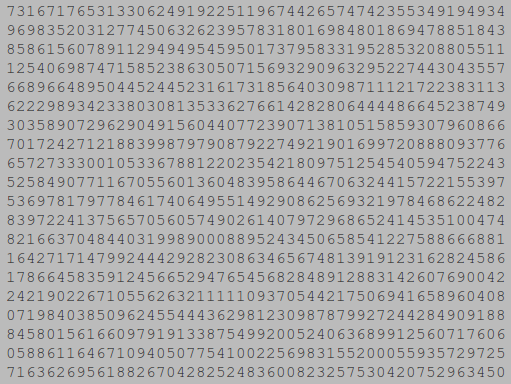
\includegraphics[scale = 0.52]{pic/008.png}
\end{center}
\end{figure}


\noindent Find the thirteen adjacent digits in the 1000-digit number that have the greatest product. What is the value of this product?
\end{prob}

\begin{sol}
Brute force.
\code{code/008.c}
\end{sol}

\section{Problem 009 - Special Pythagorean triplet}
\begin{prob}
A Pythagorean triplet is a set of three natural numbers, $a < b < c$, for which,
$$a^2 + b^2 = c^2$$
For example, $3^2 + 4^2 = 9 + 16 = 25 = 5^2$.

\noindent\\ There exists exactly one Pythagorean triplet for which $a + b + c = 1000$.
Find the product $abc$.
\end{prob}
\begin{sol}
It is known that Pythagorean triplet takes form of
$$(m^2 - n^2, 2mn, m^2 + n^2)$$
therefore, $2m^2 + 2mn = 1000$ only has one solution such that $m > n$.
\begin{eqnarray}
m^2 + m < m(m + n) = 500 < 2 m ^2
\end{eqnarray}
then $23 > m > 15$, there is only one solution $m = 20, n = 5$.
\end{sol}


\section{Problem 010 - Summation of primes}
\begin{prob}
The sum of the primes below 10 is 2 + 3 + 5 + 7 = 17.
Find the sum of all the primes below two million.
\end{prob}
\begin{sol}
Brute force. Use sieve algorithm to find all the prime numbers, and sum them up.
\code{code/010.c}
\end{sol}
\newpage
\section{Problem 011 - Largest product in a grid}
\begin{prob}
In the $20\times20$ grid below, four numbers along a diagonal line have been marked in red.
\begin{figure}[htb]
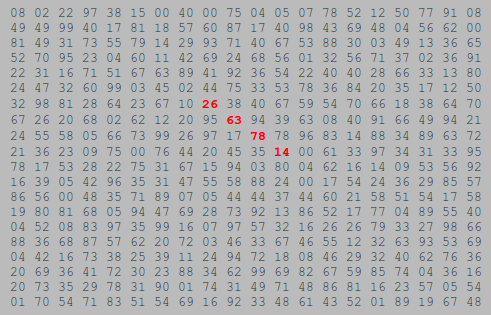
\includegraphics[scale = 0.73]{pic/010.png}
\end{figure}
\noindent\\The product of these numbers is $26 \times 63 \times 78 \times 14 = 1788696$.

\noindent\\What is the greatest product of four adjacent numbers in the same direction (up, down, left, right, or diagonally) in the $20 \times 20$ grid?
\end{prob}

\begin{sol}
Brute force.
\code{code/011.c}
\end{sol}

\newpage
\section{Problem 012 - Highly divisible triangular number}
\begin{prob}
\begin{figure}[htb!]
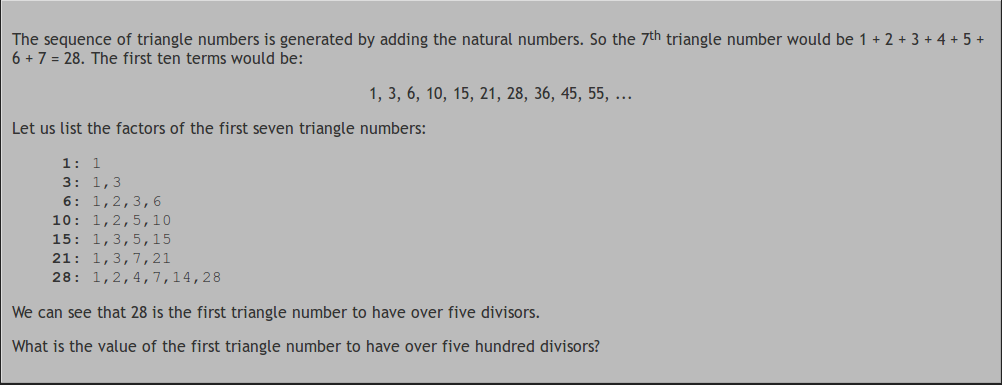
\includegraphics[scale = 0.4]{pic/012.png}
\end{figure}
\end{prob}
\begin{sol}
Brute force.
\code{code/012.c}
\end{sol}

\section{Problem 013 - Large sum}
\begin{prob}
Work out the first ten digits of the sum of the following one-hundred 50-digit numbers. \href{https://projecteuler.net/problem=13}{See data here.}
\end{prob}
\begin{sol}
The quick way is to use double type to save the numbers as $\overline{a.bcdefgh\dots}$, though machine error will only give limited accuracy around $10^{-15}$, but it is more than enough, when converting back into integer, be careful of possible overflow.
\code{code/013.c}
\end{sol}
\newpage
\section{Problem 014 - Longest Collatz sequence}
\begin{prob}
	\begin{figure}[htb!]
		\begin{center}
			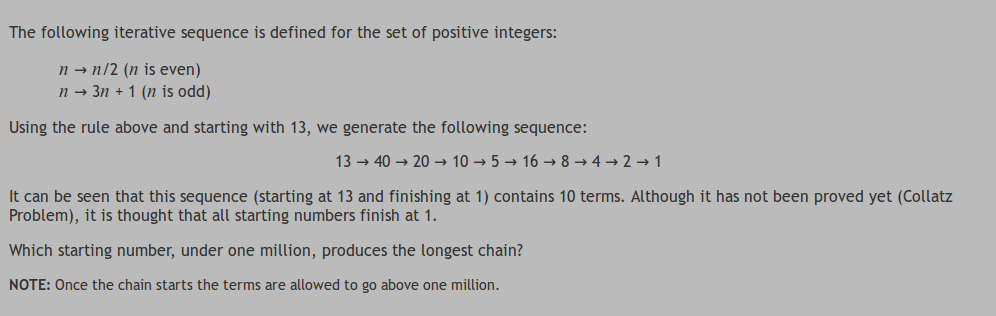
\includegraphics[scale = 0.4]{pic/014.png}
		\end{center}
	\end{figure}
\end{prob}

\begin{sol}
Brute force. Calculate the length of sequence for each start.
\code{code/014.c}
\end{sol}
\newpage
\section{Problem 015 - Lattice paths}
\begin{prob}
	\begin{figure}[htb!]
		\begin{center}
			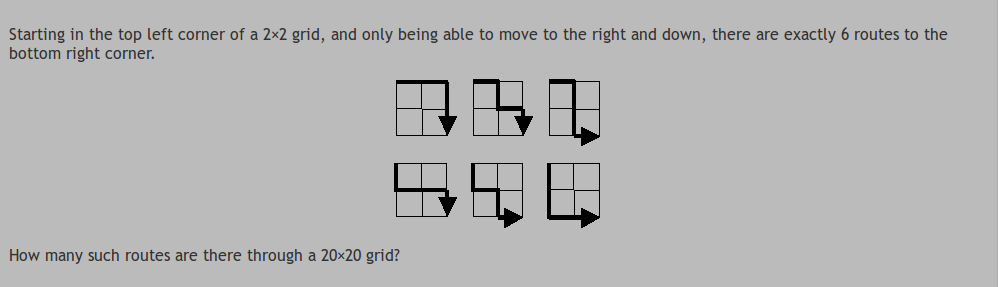
\includegraphics[scale = 0.4]{pic/015.png}
		\end{center}
	\end{figure}
\end{prob}

\begin{sol}
Suppose $f(m,n)$ represents the number of path for lattice $m \ times n$, then it is easy to observe:
$$f(m, n) = f(m - 1, n) + f(m, n - 1)$$
and $f(m, 0) = 1$, $f(0, n) = 1$. 
On the other hand, we only have $m$ steps moving right, and $n$ steps down. Thus it is equivalent to say we choose $m$ steps out of $(m + n)$ steps to move right, the rest are for moving down, which gives ${m + n}\choose m $.

\noindent \\For this problem 
$${40 \choose 20} = \frac{40!}{20! 20!} = \frac{40 \times 39 \times\dots 21}{20 \times 19\times \dots 1}$$

\noindent \\Using \texttt{long long} type should be enough to calculate.
\end{sol}
\section{Problem 016 - Power digit sum}
\begin{prob}
\begin{figure}[htb!]
	\begin{center}
	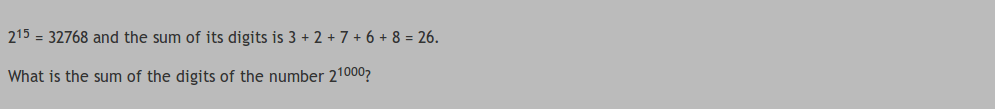
\includegraphics[scale = 0.4]{pic/016.png}
	\end{center}
\end{figure}
\end{prob}

\begin{sol}
Brute force using \texttt{BigInt} is extremely easy, since it can display all digits (around 300) of $2^{1000}$, otherwise string addition is required.
\code{code/016.c}
\end{sol}
\section{Problem 017 - Number letter counts}
\begin{prob}
	\begin{figure}[htb!]
		\begin{center}
			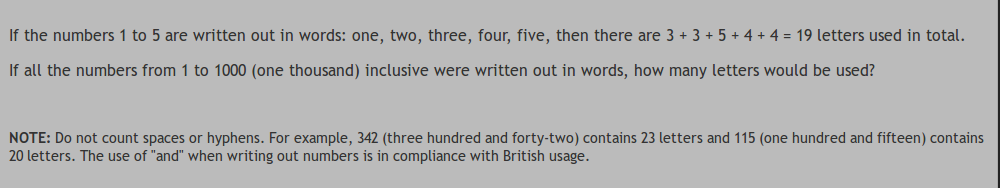
\includegraphics[scale = 0.4]{pic/017.png}
		\end{center}
	\end{figure}
\end{prob}
\begin{sol}
Brute force, no other methods.
\end{sol}
\section{Problem 018 - Maximum path sum I}
\begin{prob}
	\begin{figure}[htb!]
		\begin{center}
			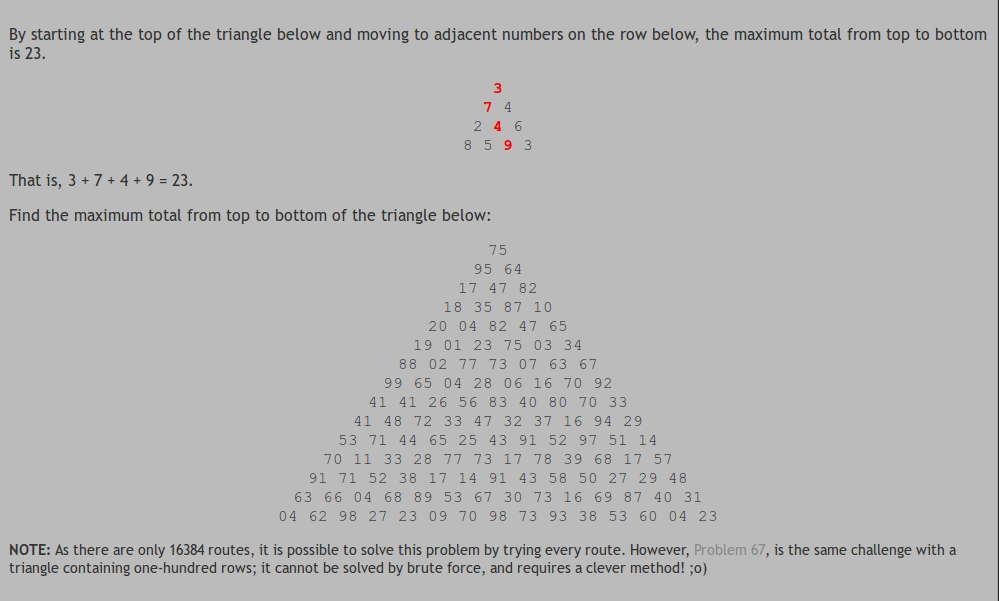
\includegraphics[scale = 0.4]{pic/018.png}
		\end{center}
	\end{figure}
\end{prob}

\begin{sol}
It is a DP problem from bottom to top.
\code{code/018.py}
\end{sol}
\section{Problem 019 - Counting Sundays}
\begin{prob}
	\begin{figure}[htb!]
		\begin{center}
			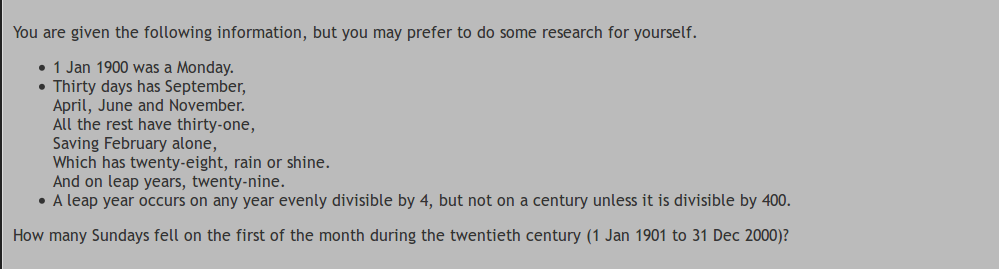
\includegraphics[scale = 0.4]{pic/019.png}
		\end{center}
	\end{figure}
\end{prob}
\begin{sol}
Brute force with library \texttt{datetime} from \texttt{Python} is straightforward.
\code{code/019.py}
\end{sol}
\section{Problem 020 - Factorial digit sum}
\begin{prob}
	\begin{figure}[htb!]
		\begin{center}
			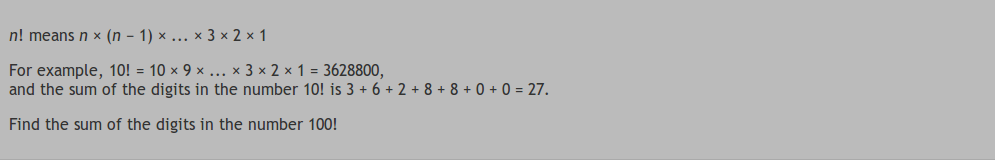
\includegraphics[scale = 0.4]{pic/020.png}
		\end{center}
	\end{figure}
\end{prob}
\begin{sol}
Brute force.
\code{code/020.py}
\end{sol}
\newpage
\section{Problem 021 -  Amicable numbers}
\begin{prob}
	\begin{figure}[htb!]
		\begin{center}
			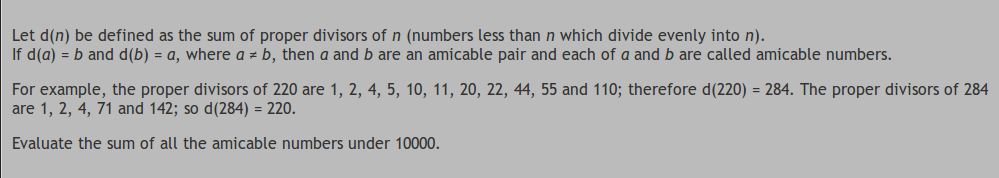
\includegraphics[scale = 0.4]{pic/021.png}
		\end{center}
	\end{figure}
\end{prob}
\begin{sol}
Brute force, check all numbers and their sum of divisors.
\code{code/021.py}
\end{sol}
\section{Problem 022 - Names scores}
\begin{prob}
	\begin{figure}[htb!]
		\begin{center}
			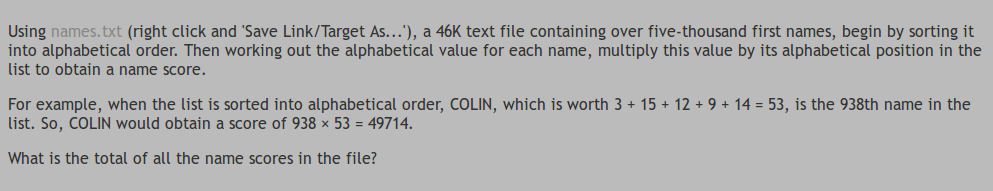
\includegraphics[scale = 0.4]{pic/022.png}
		\end{center}
	\end{figure}
\end{prob}
\begin{sol}
Brute force, using \texttt{qsort}.
\code{code/022.py}
\end{sol}
\newpage
\section{Problem 023 - Non-abundant sums}
\begin{prob}
	\begin{figure}[htb!]
		\begin{center}
			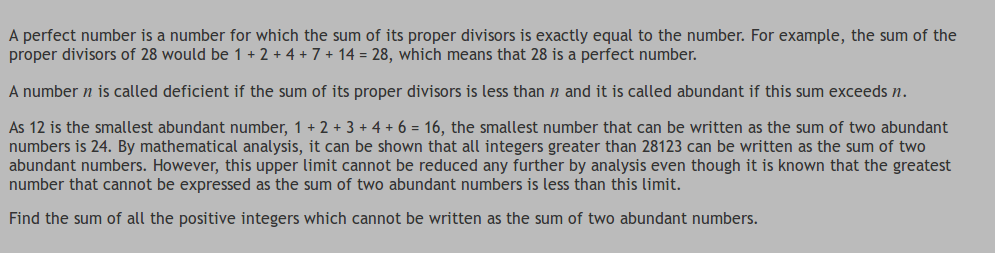
\includegraphics[scale = 0.4]{pic/023.png}
		\end{center}
	\end{figure}
\end{prob}
\begin{sol}
Brute force. Nested loop to check whether a number can be written as a sum of two abundant number.
\code{code/023.c}
\end{sol}
\section{Problem 024 - Lexicographic permutations}
\begin{prob}
	\begin{figure}[htb!]
		\begin{center}
			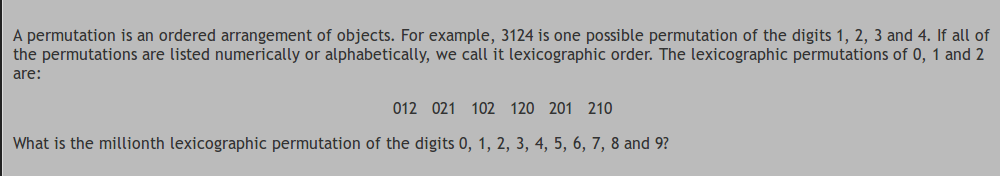
\includegraphics[scale = 0.4]{pic/024.png}
		\end{center}
	\end{figure}
\end{prob}
\begin{sol}
Not necessary to call \texttt{next\_permutation} million times. 
\code{code/024.py}
\end{sol}
\newpage
\section{Problem 025 - 1000-digit Fibonacci number}
\begin{prob}
	\begin{figure}[htb!]
		\begin{center}
			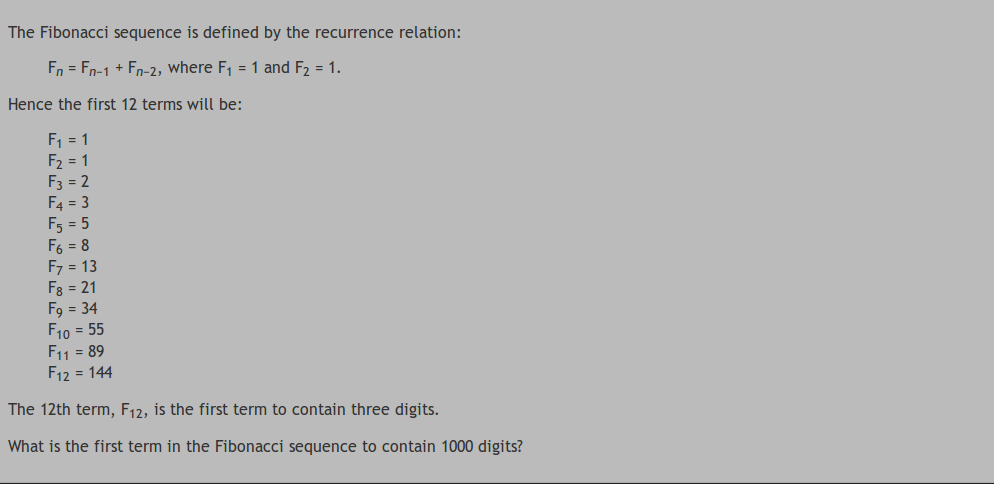
\includegraphics[scale = 0.4]{pic/025.png}
		\end{center}
	\end{figure}
\end{prob}
\begin{sol}
Brute force, just use $O(\log n)$ time complexity to get the $n^{\mathrm{th}}$ Fibonacci number. Or better
Since we know the $n^{th}$ is rounding following expression
\begin{equation}
F_n \sim \dfrac{1}{\sqrt{5}}(\phi^n)\ge 10^{999}
\end{equation}
then 
$$n \ge \dfrac{\log(5)/2 + 999 \log 10}{\log \phi} \sim 4781.8$$
\end{sol}
\chapter{LEVEL 2 @Problem 26 - 50}
\begin{chapquote}{Paul Dirac}
	``God used beautiful mathematics in creating the world.''
\end{chapquote}

\section{Problem 026 - Reciprocal cycles}
\begin{prob}
	\begin{figure}[htb!]
		\begin{center}
			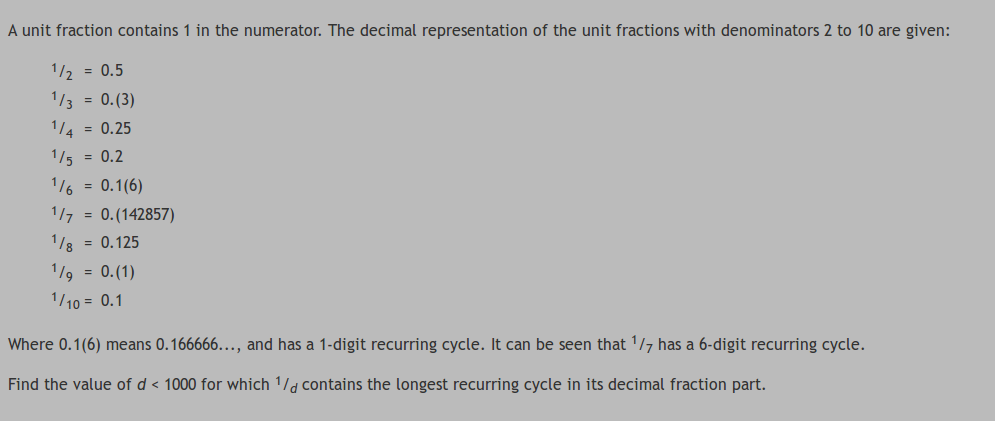
\includegraphics[scale = 0.4]{pic/026.png}
		\end{center}
	\end{figure}
\end{prob}
\begin{sol}
If $t$ is the period for number $p$, then
\begin{eqnarray}
10^{s + t} \equiv 10^s \mod p
\end{eqnarray}
If $p$ is relative prime with $2, 5$, then the above expression can be reduced to
\begin{eqnarray}
10^t \equiv 1 \mod p
\end{eqnarray}
Then brute force.
\code{code/026.py}
\end{sol}

\section{Problem 027 - Quadratic primes}
\begin{prob}
	\begin{figure}[htb!]
		\begin{center}
			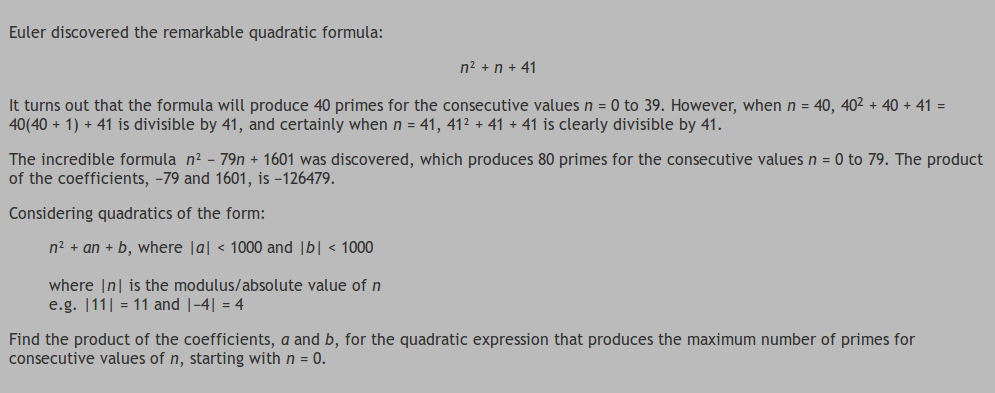
\includegraphics[scale = 0.4]{pic/027.png}
		\end{center}
	\end{figure}
\end{prob}
\begin{sol}
Brute force. But we know $b$ is a prime number between $0$ to $999$. Also we can see that when $n = b$, the result must be a compound, thus $n$ only goes from $0$ to at most $b - 1$.
\code{code/027.c}
\end{sol}

\section{Problem 028 - Number spiral diagonals}
\begin{prob}
	\begin{figure}[htb!]
		\begin{center}
			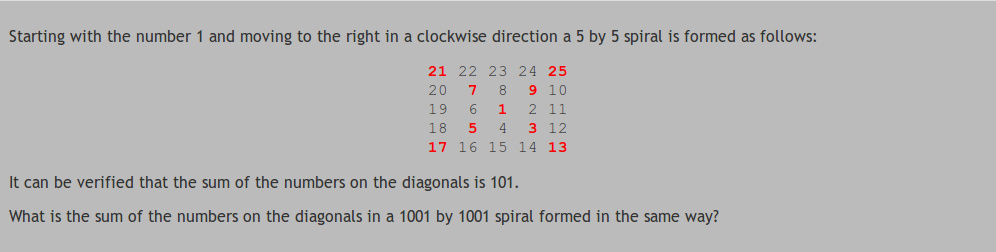
\includegraphics[scale = 0.4]{pic/028.png}
		\end{center}
	\end{figure}
\end{prob}
\begin{sol}
Deducing the formula directly may take time. We can prove that on each layer, the increment is linear to $n$, that means each layer has a sum as quadratic polynomial in $n$.
 That means the formula will take form as a cubic polynomial $f(n)$ in $n$, with $f(1) = 1, f(3) = 25, f(5) = 101, f(7) = 261$.

\begin{equation}
\begin{pmatrix}
1 & 1 & 1 & 1\\
81 & 27 & 3 & 1\\
125 & 25 & 5 & 1\\
343 & 49 & 7 & 1 
\end{pmatrix} 
\begin{pmatrix}
a\\b\\c\\d
\end{pmatrix}
 = \begin{pmatrix}
1\\25\\101\\261
\end{pmatrix}
\end{equation}
gives 
$f(n) = \dfrac{1}{6}(4 n^3 + 3n^2 + 8 n - 9)$
\end{sol}

\section{Problem 029 - Distinct powers}
\begin{prob}
	\begin{figure}[htb!]
		\begin{center}
			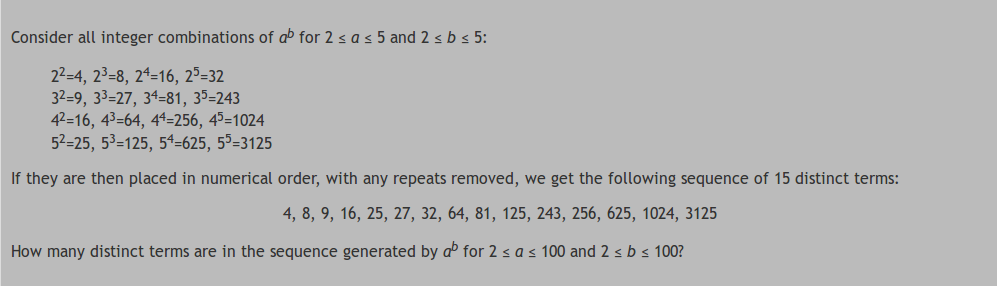
\includegraphics[scale = 0.4]{pic/029.png}
		\end{center}
	\end{figure}
\end{prob}
\begin{sol}
Brute force with \texttt{Python} one liner!
\code{code/029.py} 
\end{sol}

\section{Problem 030 - Digit fifth powers}
\begin{prob}
	\begin{figure}[htb!]
		\begin{center}
			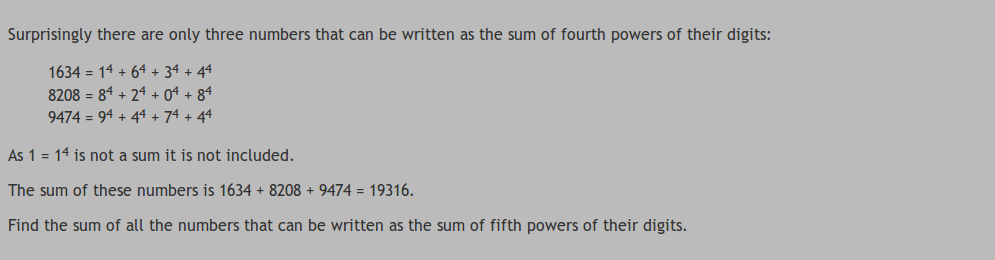
\includegraphics[scale = 0.4]{pic/030.png}
		\end{center}
	\end{figure}
\end{prob}
\begin{sol}
Brute force, since the largest number will not exceed $5 \cdot 9 ^5$.
\code{code/030.py}
\end{sol}

\section{Problem 031}
\begin{prob}
	\begin{figure}[htb!]
		\begin{center}
			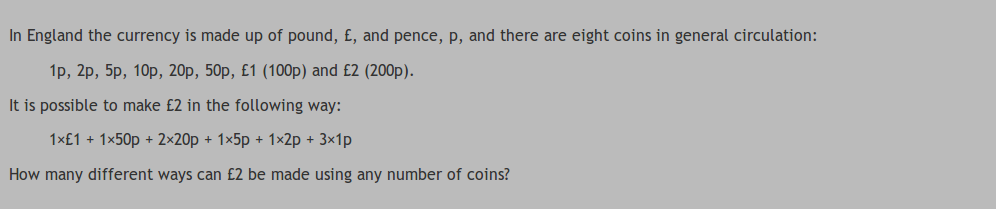
\includegraphics[scale = 0.4]{pic/031.png}
		\end{center}
	\end{figure}
\end{prob}

\begin{sol}
Consider the generating function 
$$\dfrac{1}{ (1 - x)(1 - x^2)(1 - x^5)(1 - x^{10})(1 - x^{20})(1 - x^{50})(1 - x^{100})(1 - x^{200})}$$
We simply need to find out the coefficient of $x^{200}$. To avoid long division, we can use 
$$\dfrac{1 - x ^ {201}}{1 - x} \dfrac{1 - x ^ {202}}{1 - x^2} \dfrac{1 - x^{205}}{1 - x^5} \dfrac{1 - x ^ {210}}{1 - x ^{10}}\dfrac{1 - x^{220}}{1 - x^{20}}\dfrac{1 - x^{250}}{1 - x^{50}} \dfrac{1 - x^{300}}{1 - x^{100}}\dfrac{1 - x^{400}}{1 - x^{200}}$$
instead, that will simply require multiplication of polynomials.
\vspace{1cm}
\code{code/031.py}
\end{sol}
\section{Problem 032 - Pandigital products}
\begin{prob}
	\begin{figure}[htb!]
		\begin{center}
			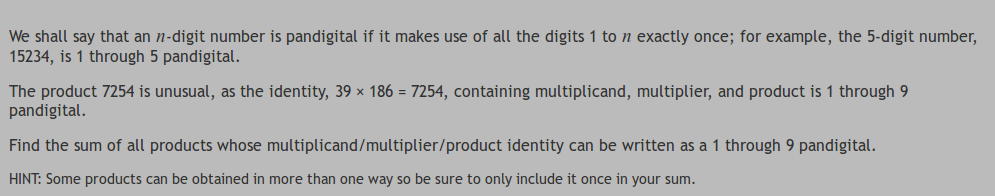
\includegraphics[scale = 0.4]{pic/032.png}
		\end{center}
	\end{figure}
\end{prob}
\begin{sol}
It is easy to show there are only two possible cases:
\begin{eqnarray}
\overline{a} \times \overline{bcde} = \overline{fghi}\\
\overline{ab}\times \overline{cde} = \overline{fghi}
\end{eqnarray}
For the first case, there are $630$ choices at most. For the second, there are $1260$ combinations.
\code{code/032.py}
\end{sol}

\section{Problem 033}
\begin{prob}
	\begin{figure}[htb!]
		\begin{center}
			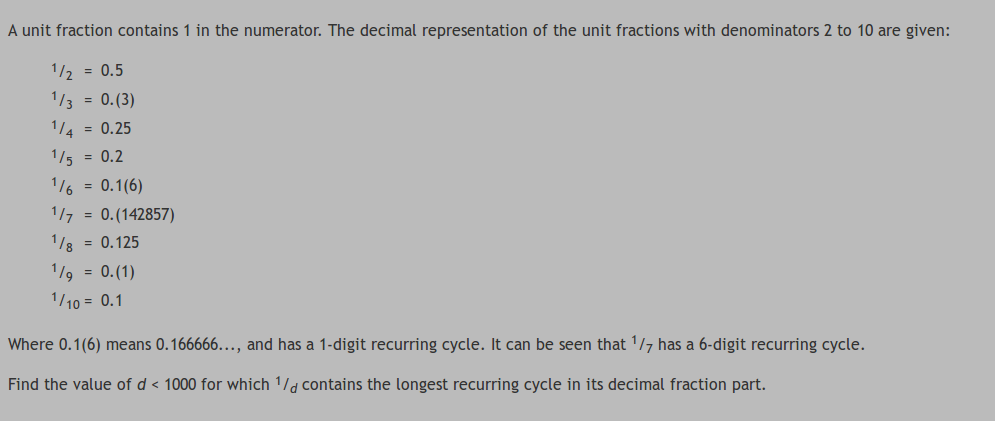
\includegraphics[scale = 0.4]{pic/026.png}
		\end{center}
	\end{figure}
\end{prob}
\section{Problem 034}
\begin{prob}
	\begin{figure}[htb!]
		\begin{center}
			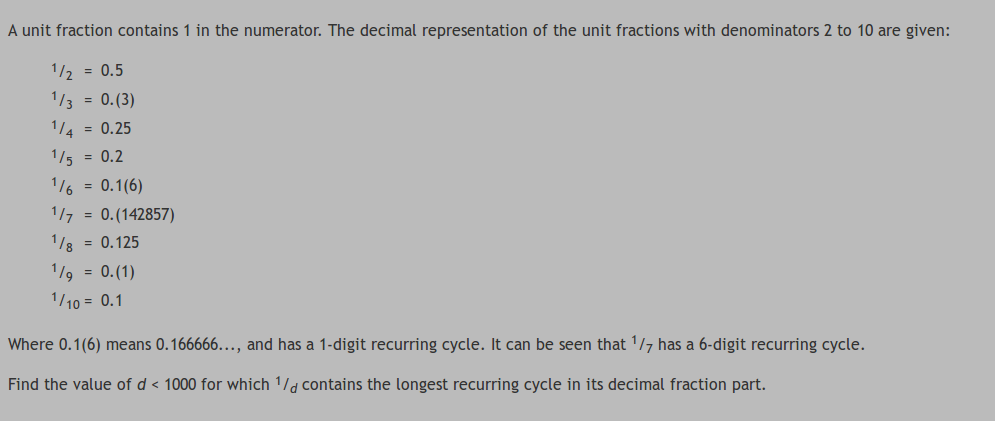
\includegraphics[scale = 0.4]{pic/026.png}
		\end{center}
	\end{figure}
\end{prob}
\section{Problem 035}
\begin{prob}
	\begin{figure}[htb!]
		\begin{center}
			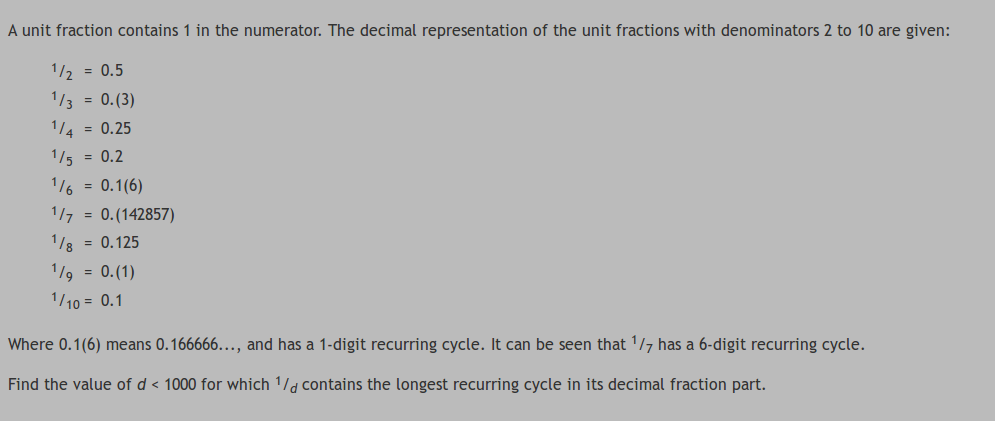
\includegraphics[scale = 0.4]{pic/026.png}
		\end{center}
	\end{figure}
\end{prob}
\section{Problem 036}
\begin{prob}
	\begin{figure}[htb!]
		\begin{center}
			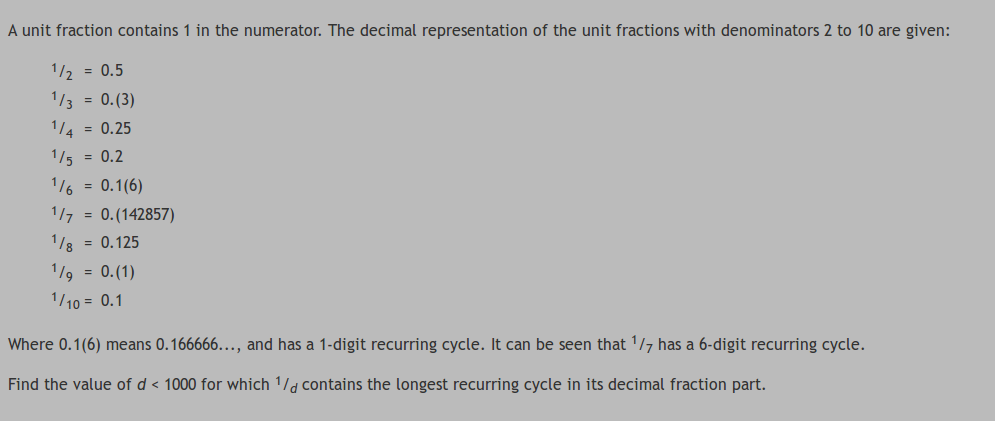
\includegraphics[scale = 0.4]{pic/026.png}
		\end{center}
	\end{figure}
\end{prob}
\section{Problem 037}
\begin{prob}
	\begin{figure}[htb!]
		\begin{center}
			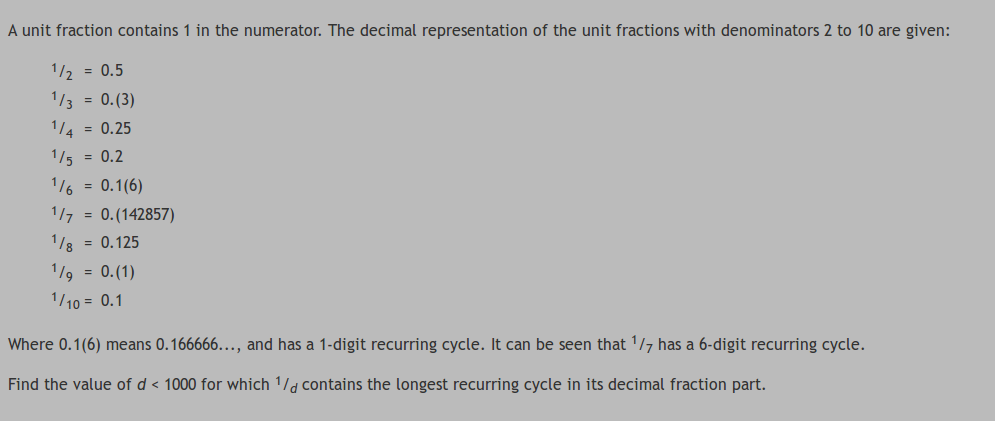
\includegraphics[scale = 0.4]{pic/026.png}
		\end{center}
	\end{figure}
\end{prob}
\section{Problem 038}
\begin{prob}
	\begin{figure}[htb!]
		\begin{center}
			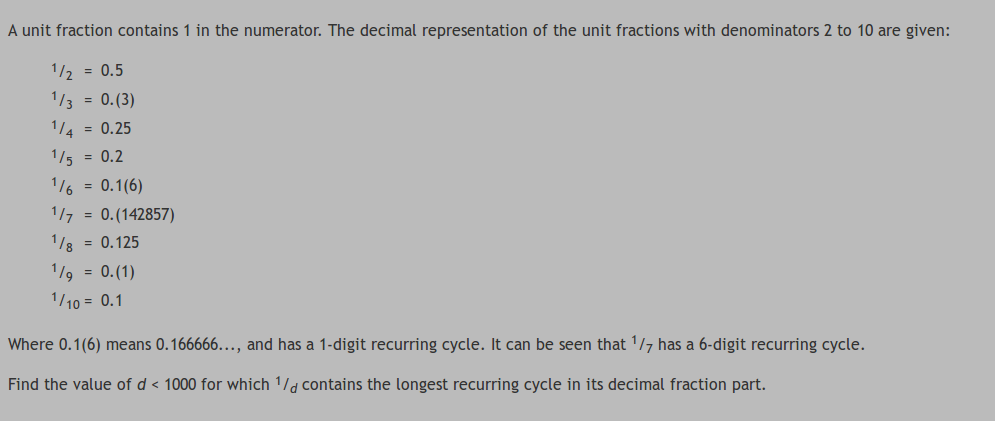
\includegraphics[scale = 0.4]{pic/026.png}
		\end{center}
	\end{figure}
\end{prob}
\section{Problem 039}
\begin{prob}
	\begin{figure}[htb!]
		\begin{center}
			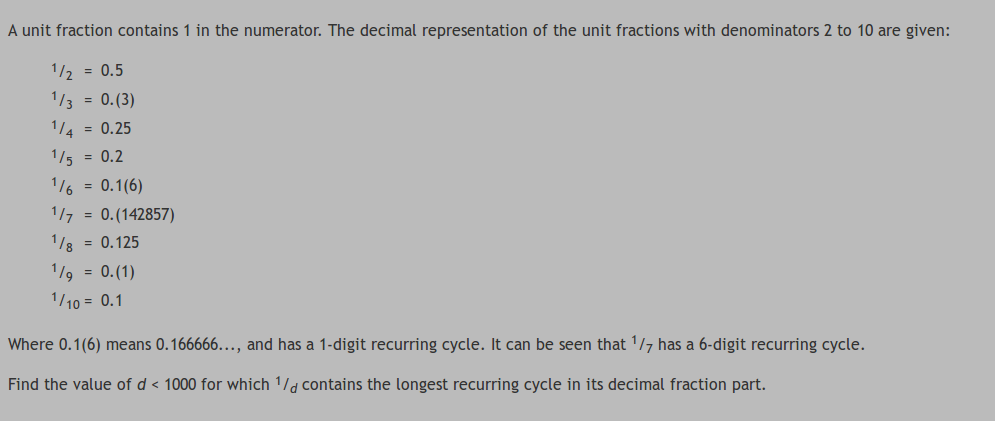
\includegraphics[scale = 0.4]{pic/026.png}
		\end{center}
	\end{figure}
\end{prob}
\section{Problem 040}
\begin{prob}
	\begin{figure}[htb!]
		\begin{center}
			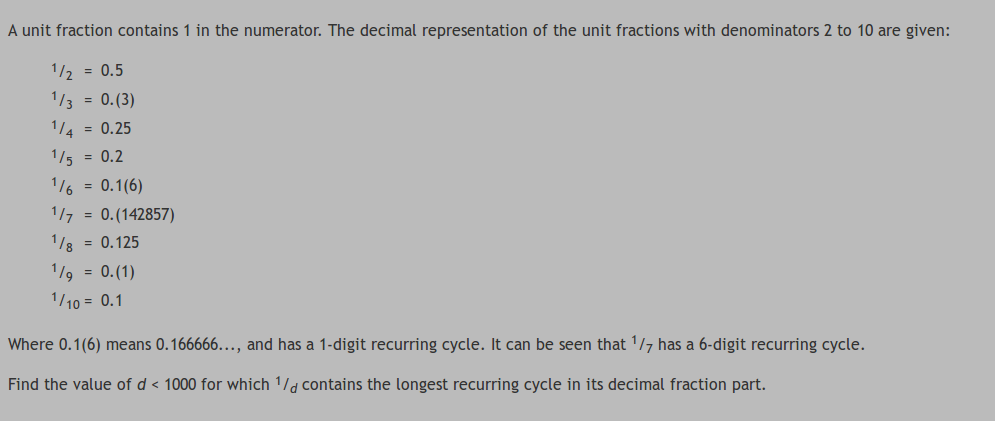
\includegraphics[scale = 0.4]{pic/026.png}
		\end{center}
	\end{figure}
\end{prob}
\chapter{LEVEL 3 @Problem 51 - 75}
\section{Problem 051}
\begin{prob}
\end{prob}
\chapter{LEVEL 4 @Problem 76 - 100}
\section{Problem 076}
\begin{prob}
\end{prob}

\chapter{LEVEL 5 @Problem 101 - 125}
\section{Problem 101}
\begin{prob}
\end{prob}
\chapter{LEVEL 6 @Problem 126 - 150}
\section{Problem 126}
\begin{prob}
\end{prob}
\chapter{LEVEL 7 @Problem 151 - 175}
\section{Problem 051}
\begin{prob}
\end{prob}
\chapter{LEVEL 8 @Problem 176 - 200}
\section{Problem 051}
\begin{prob}
\end{prob}
\chapter{LEVEL 9 @Problem 201 - 225}
\section{Problem 051}
\begin{prob}
\end{prob}
\chapter{LEVEL 10 @Problem 226 - 250}
\section{Problem 051}
\begin{prob}
\end{prob}
\chapter{LEVEL 11 @Problem 251 - 275}
\section{Problem 051}
\begin{prob}
\end{prob}
\chapter{LEVEL 12 @Problem 276 - 300}
\section{Problem 051}
\begin{prob}
\end{prob}
\chapter{LEVEL 13 @Problem 301 - 325}
\section{Problem 301}
\begin{prob}
\end{prob}
\chapter{LEVEL 14 @Problem 326 - 350}
\section{Problem 326}
\begin{prob}
\end{prob}
\chapter{LEVEL 15 @Problem 351 - 375}
\section{Problem 351}
\begin{prob}
\end{prob}
\chapter{LEVEL 16 @Problem 376 - 400}
\section{Problem 051}
\begin{prob}
\end{prob}

\chapter{LEVEL 17 @Problem 401 - 425}
\section{Problem 401}
\begin{prob}
\end{prob}
\chapter{LEVEL 18 @Problem 426 - 450}
\section{Problem 426}
\begin{prob}
\end{prob}

\chapter{LEVEL 19 @Problem 451 - 475}
\section{Problem 451}
\begin{prob}
\end{prob}
\chapter{LEVEL 19+ @Problem 475+}
\section{Problem 476}
\begin{prob}
\end{prob}

\section{Problem 479 - Roots on the Rise}
\begin{prob}
	\begin{figure}[htb!]
		\begin{center}
			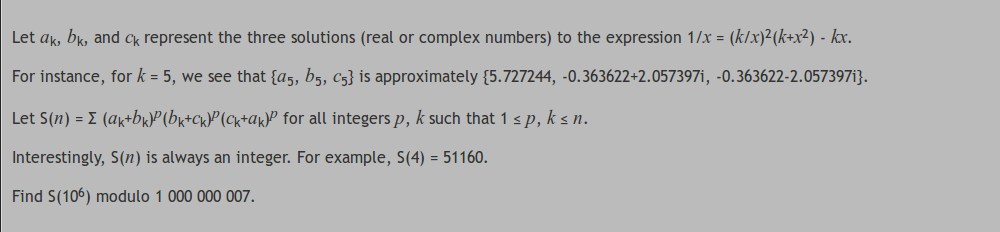
\includegraphics[scale = 0.4]{pic/479.png}
		\end{center}
	\end{figure}
\end{prob}
\begin{sol}
By Vieta's formulas, $a_k + b_k + c_k = k$, $a_kb_k + b_kc_k + c_ka_k = 1/k$, $a_kb_kc_k = k^2$.
\begin{eqnarray}
(a_k + b_k)(b_k + c_k)(c_k + a_k) = (a_k + b_k + c_k)(a_kb_k + b_kc_k + c_ka_k) -a_kb_kc_k = 1 - k^2.
\end{eqnarray}
Then we just have to evaluate
\begin{eqnarray}
\sum_{k = 1}^n ((1 - k^2)^{n + 1} - (1 - k^2))/(- k^2) \mod p
\end{eqnarray}
where 
\begin{eqnarray}
(-k^2)^{-1} \equiv (-k^2)^{p-2} \mod{p}
\end{eqnarray}
Using \texttt{ModPow} with \texttt{BigInt} will be efficient, in \texttt{Python}, simply use \texttt{pow} with the third argument.
\code{code/479.py}
\end{sol}
\section{Problem 500}
\begin{prob}
\end{prob}
\end{document}
